\documentclass{beamer} % Use handout to get rid of repeated slides
\usetheme{AnnArbor}
\usecolortheme{default}
\usefonttheme{professionalfonts}
\usepackage{mathpazo}
\usepackage{listings}
\usepackage{xcolor}

% Define colors
\definecolor{myred}{RGB}{163,0,0}
\definecolor{ttcolor}{RGB}{0,0,1}%{RGB}{163,0,0}
\definecolor{mygray}{RGB}{248,249,250} 
\definecolor{mygreen1}{RGB}{0,96,0}
\definecolor{mygreen2}{RGB}{229,239,229}
\definecolor{aristotelgreen}{HTML}{008A44}
\definecolor{aristotelred}{HTML}{9E0101}
\definecolor{aristotelgrey}{HTML}{2E2E2E}
\definecolor{aristoteldarkred}{HTML}{500101}
\definecolor{aristotelorange}{HTML}{FF8C00}

\setbeamertemplate{theorem}[ams style]
\setbeamertemplate{theorems}[numbered]

\usepackage{etoolbox}
\usepackage{amsmath}

\undef{\definition}
\theoremstyle{definition}
\newtheorem{definition}{\translate{Definition}}
\hypersetup{
	colorlinks=true,
	linkcolor=aristotelorange,   % color for normal internal links
	citecolor=aristotelgreen,   % color for citation links
	urlcolor=aristotelgreen      % color for external links
}

\setbeamercolor{palette primary}{bg=aristotelred, fg=white}
\setbeamercolor{palette secondary}{bg=aristoteldarkred, fg=white}
\setbeamercolor{palette tertiary}{bg=black, fg=white} 

\setbeamercolor{title}{fg=white, bg=aristotelred} % Title text color
\setbeamercolor{subtitle}{fg=white, bg=aristotelred} % Subtitle text color
\setbeamercolor{background canvas}{bg=aristotelgrey} % Background for content canvas
\setbeamercolor{normal text}{fg=white} % Normal text color
\setbeamercolor{titlegraphic}{bg=mygray} % Background color for title graphic area
\setbeamercolor{frametitle}{fg=white, bg=aristoteldarkred}

% Change color of numbered circles in the table of contents
\setbeamercolor{section number projected}{bg=white, fg=black}
\setbeamercolor{subsection number projected}{bg=aristotelred, fg=aristotelgrey}
\setbeamercolor{subsection number projected}{bg=aristotelorange, fg=white}


\setbeamercolor{block title}{fg=white,bg=mygreen1}
\setbeamercolor{block body}{fg=black,bg=mygreen2}


\lstdefinestyle{rstyle}%
{language=[LaTeX]TeX,
	basicstyle=\footnotesize\ttfamily,
	backgroundcolor = \color{mygray},
	commentstyle=\slshape\color{green!50!black},
	keywordstyle=\color{blue},
	identifierstyle=\color{blue},
	stringstyle=\color{orange},
	%escapechar=\#,
	rulecolor = \color{mygray}, 
	showstringspaces = false,
	showtabs = false,
	tabsize = 2,
	emphstyle=\color{red},
	frame = single} 


\begin{document}
	
	% Title page
	\title[Student Performance]{Predicting First-Year Statistics Grades}
	\subtitle{From Attendance, Honesty, and Quiz Results \\
		Cohort 2025/29}
	\author[Riste Petrov]{Riste Petrov \\ \href{mailto:riste@uni-sofia.bg}{riste@uni-sofia.bg}}
	\institute[AEEM - FEBA]{AEEM - FEBA master degree student cohort 2025/26}
	\titlegraphic{\includegraphics[scale=0.5]{/home/anonymous/Documents/Mega/ЦЕЛ/Master/1Courses/SU ENG White horizontal.pdf}}
	\date{\today}
	
	% Frame: Title Page
	\begin{frame}
		\titlepage
	\end{frame}
	
	% Frame: Table of Contents
	\begin{frame}
		\frametitle{Contents}
		\tableofcontents
	\end{frame}
	
	% Sections and Subsections
	\section{Introduction}
	
	\subsection{Hypotheses}
	\begin{frame}
		\frametitle{Hypotheses}
		\centering
		\begin{itemize}
			\item \textbf{H0}: Attendance, homework completion/timeliness, and academic honesty predict test performance more strongly than attitude toward math.
			\item \textbf{H1}: Seating proximity to higher- or lower-achieving peers affects student performance.
			\item \textbf{H2}: Lower attendance, late homework, digital submission, and low quiz scores are associated with lower final results.
		\end{itemize}
	\end{frame}
	
	\subsection{Sample}
	\begin{frame}
		\frametitle{Sample}
		\begin{itemize}
			\item 49 students enrolled in the Statistics course at University Goce Delchev (UGD) Shtip.
			\item Data collected includes attendance, quiz scores, seating positions, and honesty indicators.
			\item Limitations: Small sample size, potential biases, and measurement constraints.
		\end{itemize}
	\end{frame}
	
	\subsection{Experimental Design}
	\begin{frame}
		\frametitle{Experimental Design}
		\begin{itemize}
			\item Data collection was unobtrusive to preserve natural behavior.
			\item Quizzes administered via Google Forms; attendance and seating observed without informing students of specific hypotheses.
			\item Data aggregated into summary measures to reduce dimensionality.
		\end{itemize}
	\end{frame}
	
	\subsection{Feature Engineering}
	\begin{frame}
		\frametitle{Feature Engineering}
		\begin{itemize}
			\item Variables were summarized (means, indices) for analysis.
			\item Focused on behavioral, attendance, and seating proximity measures.
			\item Considered potential confounders such as prior math achievement.
		\end{itemize}
	\end{frame}
	
	\begin{frame}
		\frametitle{Identifiers \& Background}
		\begin{itemize}
			\item anonINDX - continuous \\
			\subitem ascending student index (1 = first); identifier and a control for random effects.
			\item GENDER - logical \\
			\subitem inferred from name: 0 = male, 1 = female
			\item HSCH - categorical [1--3] \\
			\subitem 1 general, 2 economics/law specialized, 3 other
			\item MJR - categorical [1--6]  \\
			\subitem 1 Finance, 2 Business Economics, 3 Marketing \& Management, 4 Accounting \& Audit, 5 International Economics \& Business, 6 Other
			\item atitMATH - categorical [1--6]  \\
			\subitem self‑rated attitude to math (1 = awful … 6 = favorite)
		\end{itemize}
	\end{frame}
	
	\begin{frame}
		\frametitle{Quiz \& Attendance (aggregates)}
		\begin{itemize}
			\item averQIZZ$_{1/2}$ - continuous (0–1)\\  
			\subitem average quiz score in part 1 / part 2
			\item diffQIZZ$_{1/2}$ - continuous (0–1)\\  
			\subitem change between first quiz and overall quiz average
			\item averATND$_{1/2}$ - continuous\\  
			\subitem average attendance (part 1 / part 2), built from:\\
			\subitem numP$_{1/2}$\\
			\subitem numE$_{1/2}$\\
			\subitem numQ$_{1/2}$
		\end{itemize}
	\end{frame}
	
	\begin{frame}
		\frametitle{Dishonesty \& Homework}
		\begin{itemize}
			\item DISS$_{1}$/DISS$_{2}$ - continuous  \\
			\subitem cumulative dishonesty index (DISS$_2$ = DISS$_1$ + new incidents)\\
			\subitem components (logical): honLST (falsified signature, +3), honHW (dishonest HW claim, +1), Y1 CHEAT / Y2 CHEAT (suspicious midterm behaviors, +2 each)
			\item Homework (regular)\\
			\subitem numHW$_{1/2}$ - continuous/logical: counts\\
			\subitem paperHW$_{1/2}$, lateHW$_{1/2}$ - continuous/logical: submission format and timeliness\\
			\subitem hardHW$_{1/2}$ - categorical (rescaled 0–1): perceived difficulty\\
			\item Additional HW
			\subitem additHW$_{1/2}$ - logical; lateADHW$_{1/2}$ - logical (context-specific)
		\end{itemize}
	\end{frame}
	
	\begin{frame}
		\frametitle{Seating Proximity \& Outcomes}
		\begin{itemize}
			\item PROXI25$_{1/2}$ - continuous  \\
			\subitem fraction of sessions sitting within ±2 index positions of peers below 25th percentile
			\item PROXI75$_{1/2}$ - continuous \\ 
			\subitem fraction of sessions sitting within ±2 index positions of peers above 75th percentile\\
			\subitem proximity computed from per‑session seating index (two seats ahead/behind)\\
			
			\item Outcomes
			\subitem Y1 / Y2 - continuous (0–1, scaled from 0–20 pts): midterm scores (Y1 easier; Y2 harder, dynamic assignment)\\
			\subitem Y1GROUP / Y2GROUP - group controls \\
		\end{itemize}
	\end{frame}
	
	
	\section{Results}
	
	\subsection{Modeling First Quiz Results}
	\begin{frame}
		\frametitle{Modeling First Quiz Results}
		\begin{itemize}
			\item Regression with demographic and background variables.
			\item Key variables: No significant predictors; model explains limited variance.
			\item Notable finding: Prior math achievement likely influential but unmeasured here.
		\end{itemize}
	\end{frame}
	
	\subsection{H0: Honesty vs Attitude Toward Math}
	\begin{frame}
		\frametitle{H0: Honesty vs Attitude Toward Math}
		\begin{itemize}
			\item \textbf{Main finding}: Dishonesty index negatively correlates with exam scores.
			\item \textbf{Attitude toward math}: Weak or no significant effect.
			\item \textbf{Implication}: Academic honesty is a stronger predictor than attitude.
		\end{itemize}
		\vspace{1em}
		\begin{block}{Sample Regression Result}
			\centering
			\small
			\textit{Each point increase in dishonesty index reduces scores by approximately 7.6–11.2 percentage points.}
		\end{block}
	\end{frame}
	
	% Include your regression tables here
	% Example:
	\begin{frame}
		\frametitle{Regression Results for H0}
		\begin{center}
			% Your table here, or include as figure for better formatting
			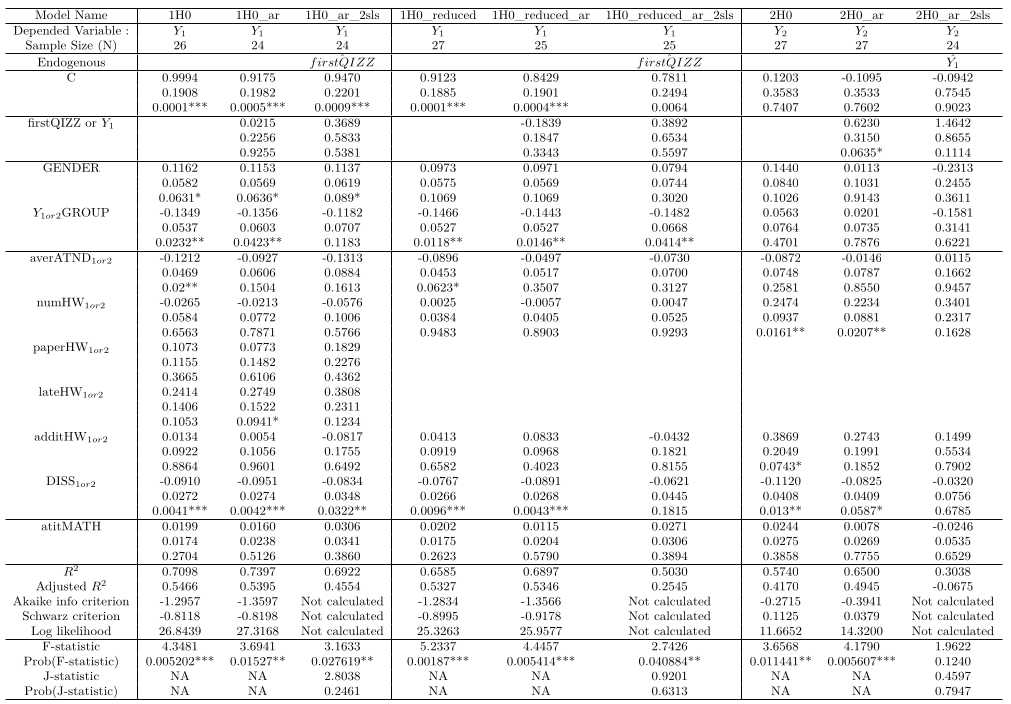
\includegraphics[width=0.85\linewidth]{h0.png}
		\end{center}
	\end{frame}
	
	\subsection{H1: Seating Proximity and Honesty}
	\begin{frame}
		\frametitle{H1: Seating Proximity and Peer Effects}
		\begin{itemize}
			\item \textbf{Key result}: Sitting near higher-achieving peers (PROXI75) positively impacts scores.
			\item \textbf{Effect persists}: Remains significant after controlling for dishonesty.
			\item \textbf{No effect}: Proximity to lower-achieving peers (PROXI25) shows no consistent impact.
			\item \textbf{Mechanism}: Evidence suggests knowledge transfer or social learning, not collusion.
		\end{itemize}
		\vspace{1em}
		% Include your detailed tables or figures here
	\end{frame}
	
	\begin{frame}
		\frametitle{Regression Results for H1 midterm 1}
		\begin{center}
			% Your table here, or include as figure for better formatting
			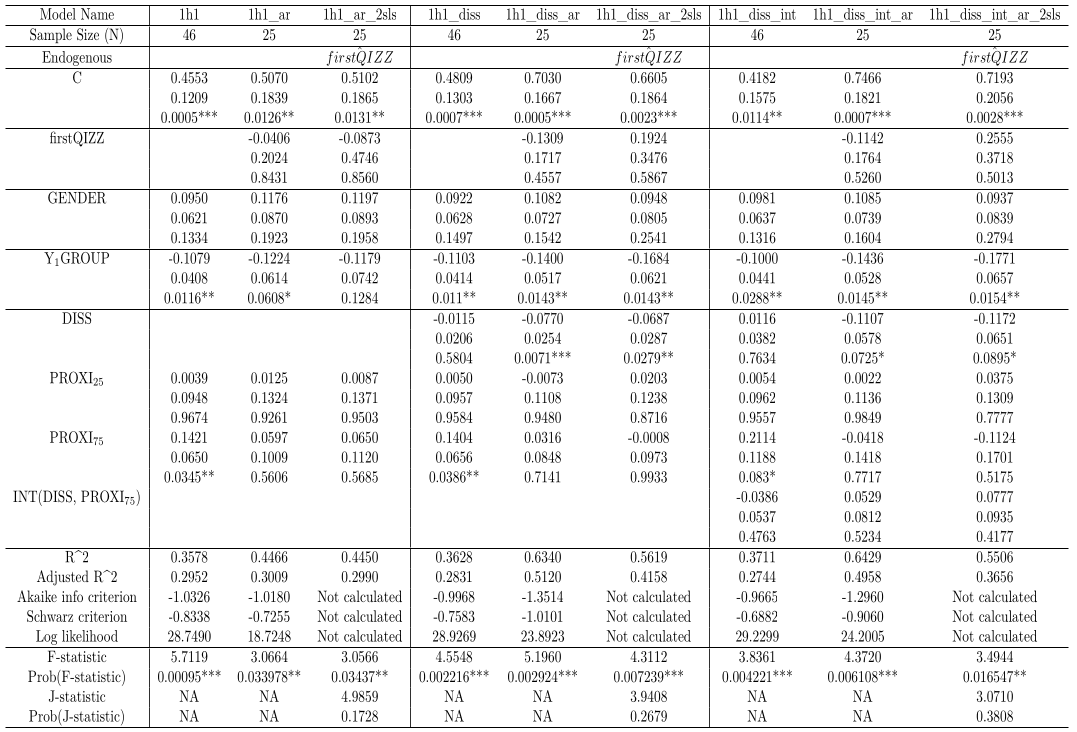
\includegraphics[width=0.85\linewidth]{h1-1.png}
		\end{center}
	\end{frame}
	
	\begin{frame}
		\frametitle{Regression Results for H1 midterm 1}
		\begin{center}
			% Your table here, or include as figure for better formatting
			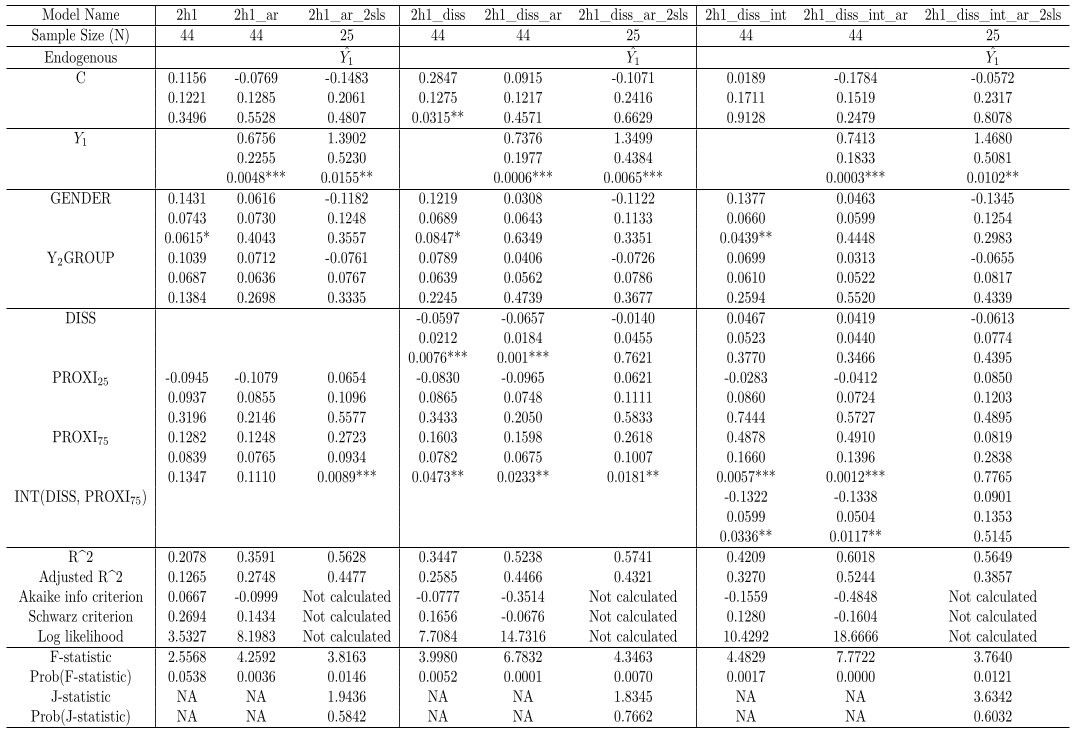
\includegraphics[width=0.85\linewidth]{h1-2.png}
		\end{center}
	\end{frame}
	
	\subsection{H2: Performance and Homework Behaviors}
	\begin{frame}
		\frametitle{H2: Homework and Performance}
		\begin{itemize}
			\item \textbf{Result}: No significant linear relationship between attendance, homework orderliness, quiz performance, and perceived difficulty.
			\item \textbf{Possible reasons}: Measurement limitations, small sample size.
			\item \textbf{Future directions}: Better objective measures, larger samples, nonlinear models.
		\end{itemize}
	\end{frame}
	
	\section{Discussion}
	\begin{frame}
		\frametitle{Discussion}
		\begin{itemize}
			\item \textbf{Main findings}: Peer proximity to higher achievers enhances performance; dishonesty correlates negatively.
			\item \textbf{Limitations}: Small sample, measurement constraints, potential biases.
			\item \textbf{Implications}: Seating arrangements could be a low-cost intervention.
			\item \textbf{Caution}: Results are suggestive; causality not definitively established.
		\end{itemize}
	\end{frame}
	
	\subsection{Limitations}
	\begin{frame}
		\frametitle{Limitations}
		\begin{itemize}
			\item Small sample size and limited external validity.
			\item Measurement issues: Homework quality, dishonesty proxies.
			\item Potential observer effects and unmeasured confounders.
			\item Lack of prior achievement data.
		\end{itemize}
	\end{frame}
	
	\subsection{Future Research}
	\begin{frame}
		\frametitle{Future Research}
		\begin{itemize}
			\item Larger, multi-cohort studies with diverse samples.
			\item Objective measures: Rubric-scored homework, prior grades.
			\item Automated participation and attention metrics.
			\item Use of panel data.
			\item Explore nonlinear and interaction effects.
		\end{itemize}
	\end{frame}
	
	% Q&A slide
	\begin{frame}
		\frametitle{Questions and Discussion}
		\begin{center}
			I appreciate your attention.\\
			\vspace{1em}
			Q \& A?
		\end{center}
	\end{frame}
	
\end{document}